\clearpage
\subsection{Architettura del sistema}
L'architettura del sistema è stata formalizzata attraverso due deployment diagram differenti: il primo, riportato in figura \ref{fig:DeplymnetDiagramNonFormale}, rappresenta il sistema tramite una notazione a stile libero, mentre il secondo, riportato in figura \ref{fig:DeplymnetDiagramFormale}, rappresenta il sistema tramite lo stile UML. In particolare, in entrambi i diagrammi è possibile identificare un pattern architetturale \textit{three thier}. All'interno del \textit{presentation layer} ci sono le applicazioni lato client che vengono utilizzate dagli attori. Nell'\textit{application layer} ci sono invece due macchine distinte:

\begin{itemize}
	\item su una macchina c'è un \textbf{Web Server Java}, che si occupa della gestione di richieste tramite protocollo \textit{HTTP/Rest};
	\item sull'altra macchina ci sono due componenti autonome, un \textbf{Data Fetcher} che si occupa di recuperare informazioni dai data server tramite API e le inserisce all'interno del database, ed un \textbf{Data Analyzer} che si occupa di effettuare delle analisi dei dati acquisiti con lo scopo di identificare possibili situazioni di emergenza.
\end{itemize}

Nel \textit{data layer} troviamo invece un database all'interno del quale sono inserite tutte le informazioni inerenti il sistema.

\begin{sidewaysfigure}[h!]
	\centering
	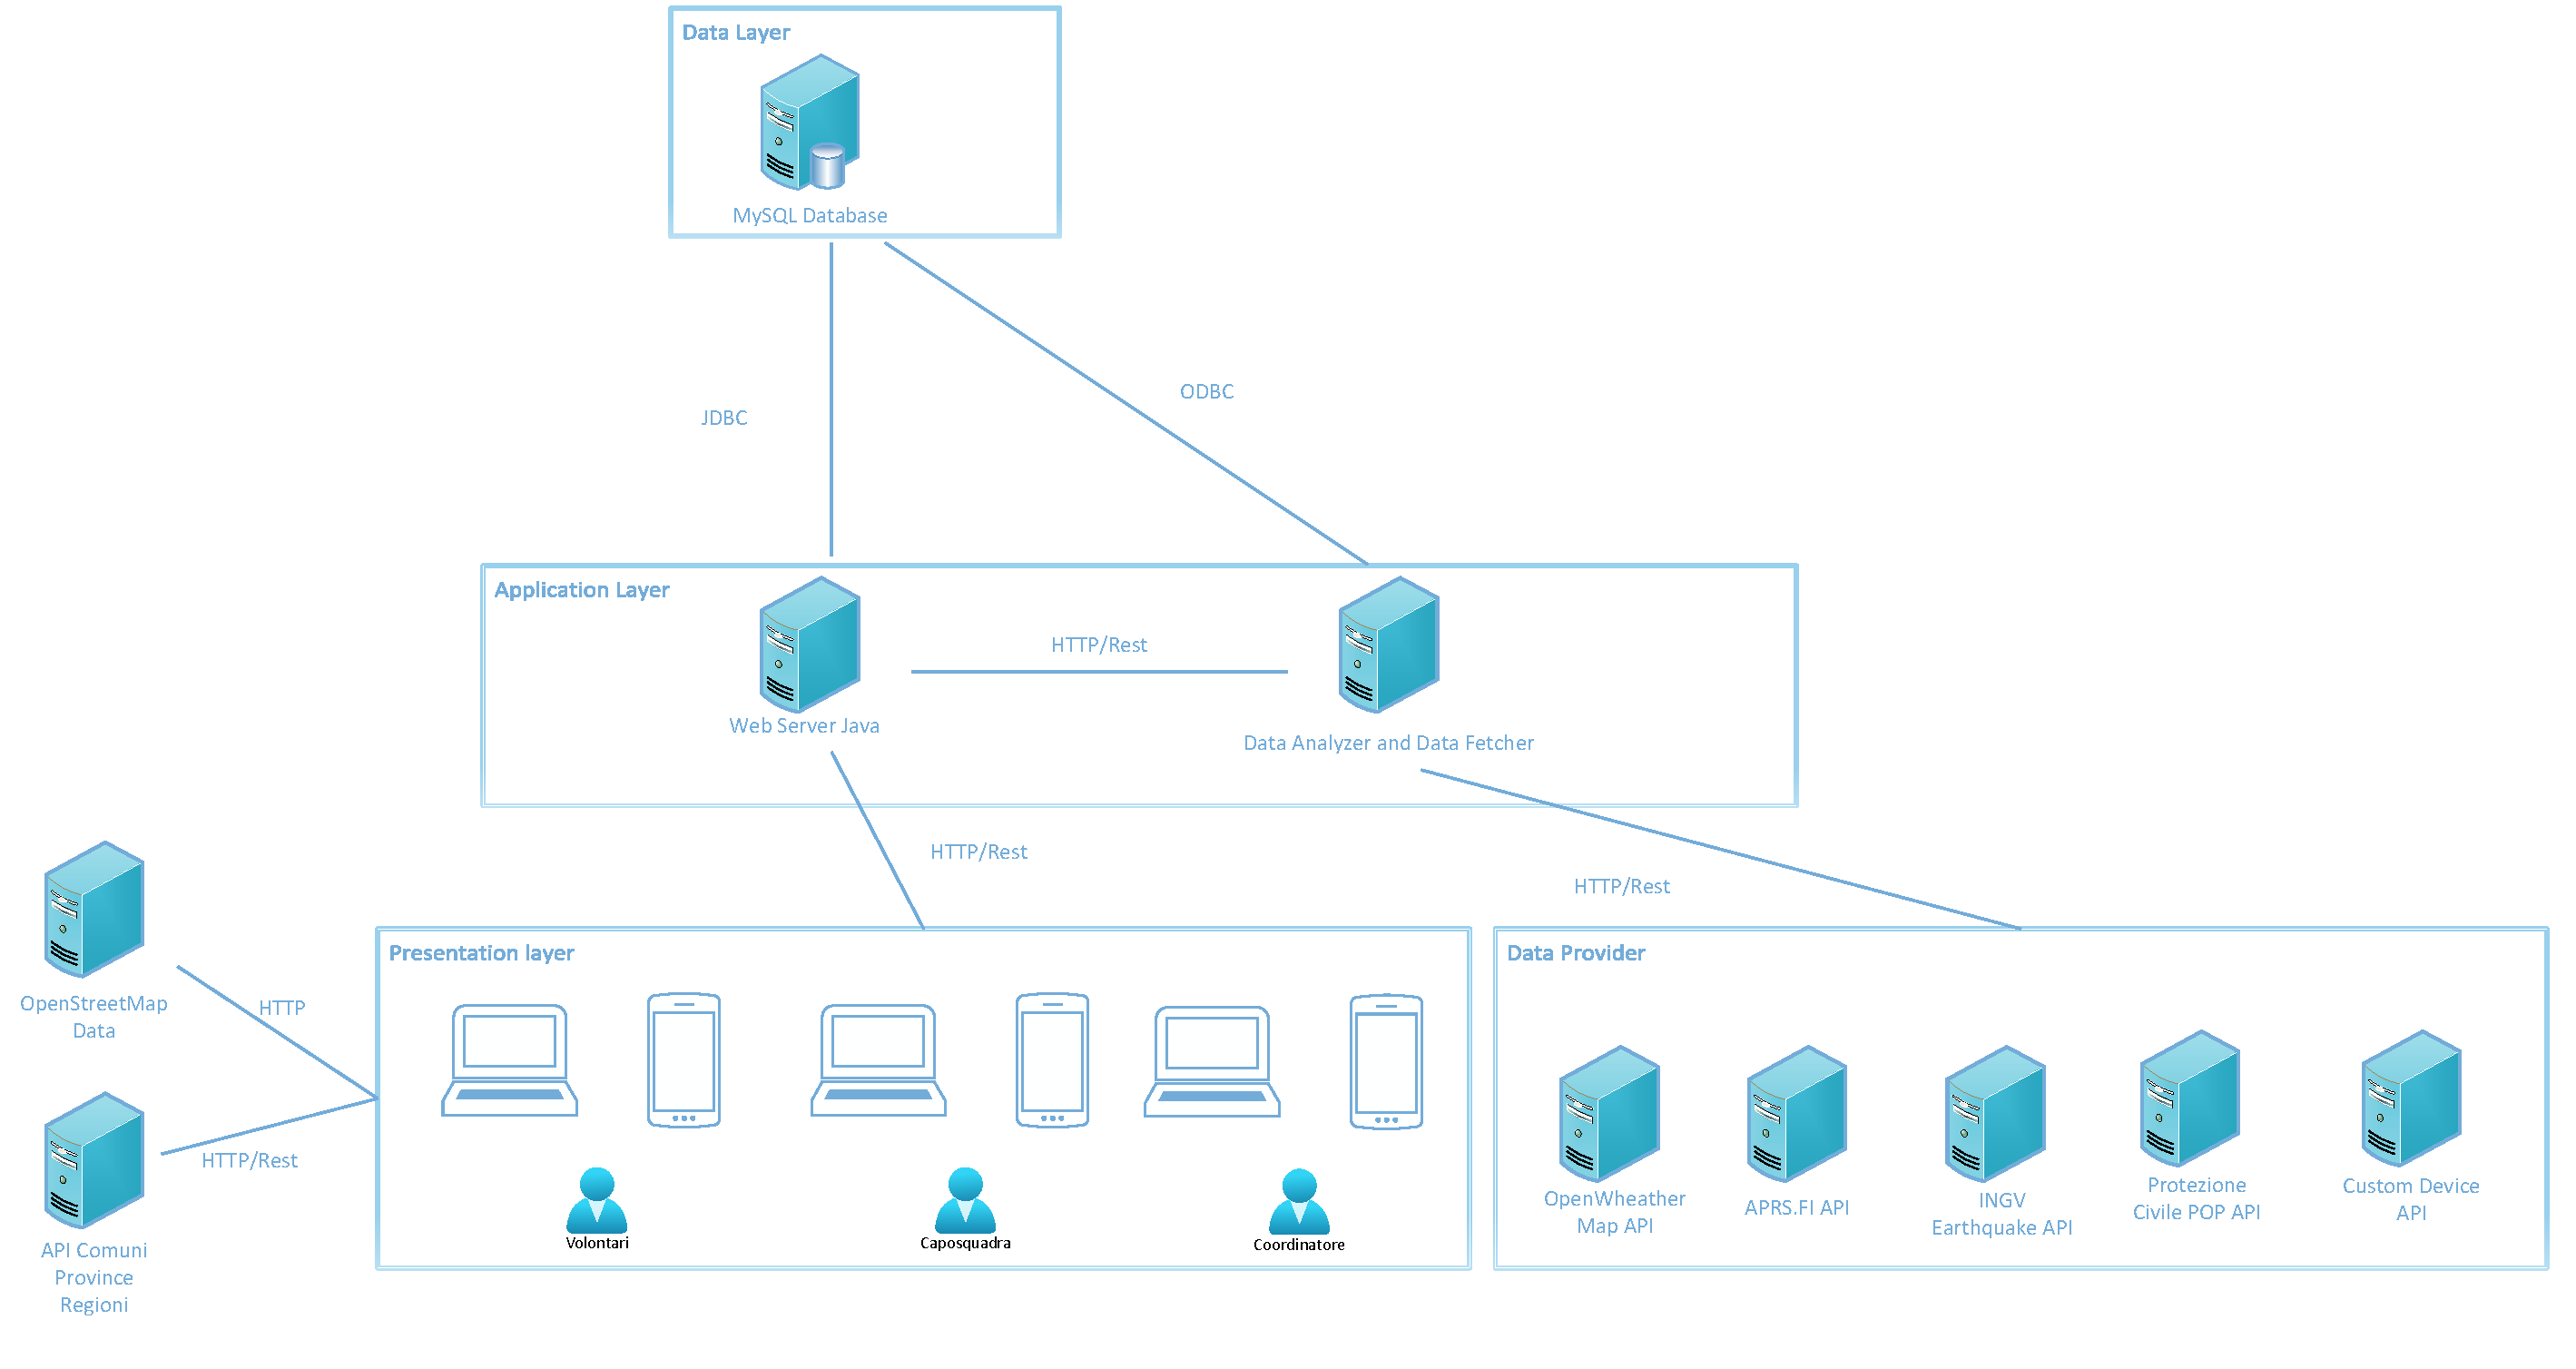
\includegraphics[width=0.9\linewidth]{OtherFiles/DeploymentDiagramNonFormale}
	\caption{Deployment diagram in stile libero.}
	\label{fig:DeplymnetDiagramNonFormale}
\end{sidewaysfigure}

\begin{sidewaysfigure}[h!]
	\centering
	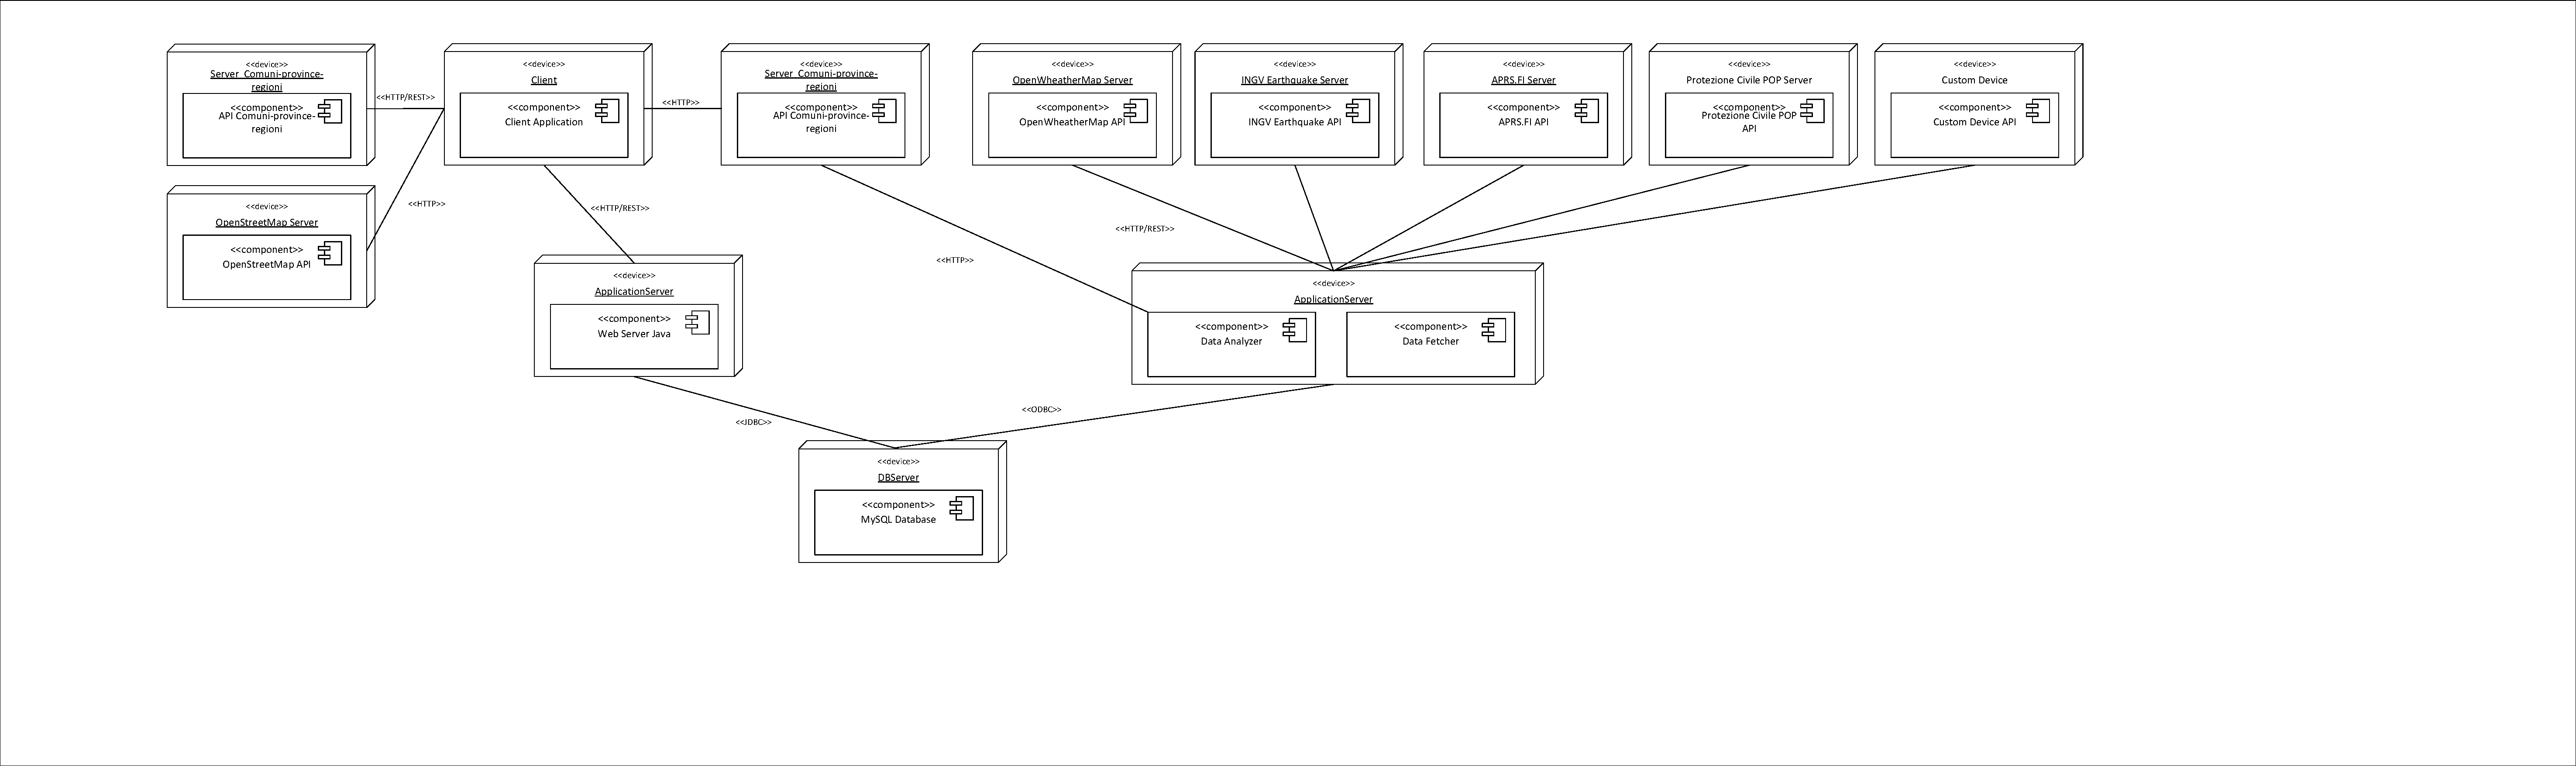
\includegraphics[width=0.9\linewidth]{OtherFiles/DeplymentDiagramFormale}
	\caption{Deployment diagram in stile UML.}
	\label{fig:DeplymnetDiagramFormale}
\end{sidewaysfigure}
